
% Cal Poly Thesis
% 
% based on UC Thesis format
%
% modified by Mark Barry 2/07.
%




\documentclass[12pt]{ucthesis}

\newif\ifpdf
\ifx\pdfoutput\undefined
    \pdffalse % we are not running PDFLaTeX
\else
\pdfoutput=1 % we are running PDFLaTeX
\pdftrue \fi

\usepackage{url}
\ifpdf

    \usepackage[pdftex]{graphicx}
    % Update title and author below...
    \usepackage[pdftex,plainpages=false,breaklinks=true,colorlinks=true,urlcolor=blue,citecolor=blue,%
                                       linkcolor=blue,bookmarks=true,bookmarksopen=true,%
                                       bookmarksopenlevel=3,pdfstartview=FitV,
                                       pdfauthor={Gregory Flanagan},
                                       pdftitle={Conceptual Requirement Validation for Architecture Design Systems},
                                       pdfkeywords={thesis, masters, cal poly}
                                       ]{hyperref}
    %Options with pdfstartview are FitV, FitB and FitH
    \pdfcompresslevel=1

\else
    \usepackage{graphicx}
\fi

\usepackage{amssymb}
\usepackage{amsmath}
\usepackage[letterpaper]{geometry}
\usepackage[overload]{textcase}
\usepackage{subfig}
\usepackage{float}


\bibliographystyle{abbrv}

\setlength{\parindent}{0.25in} \setlength{\parskip}{6pt}

\geometry{verbose,nohead,tmargin=1.25in,bmargin=1in,lmargin=1.5in,rmargin=1.3in}

\setcounter{tocdepth}{2}
\graphicspath{{fig/}}


% Different font in captions (single-spaced, bold) ------------
\newcommand{\captionfonts}{\small\bf\ssp}

\makeatletter  % Allow the use of @ in command names
\long\def\@makecaption#1#2{%
  \vskip\abovecaptionskip
  \sbox\@tempboxa{{\captionfonts #1: #2}}%
  \ifdim \wd\@tempboxa >\hsize
    {\captionfonts #1: #2\par}
  \else
    \hbox to\hsize{\hfil\box\@tempboxa\hfil}%
  \fi
  \vskip\belowcaptionskip}
\makeatother   % Cancel the effect of \makeatletter
% ---------------------------------------




\begin{document}

% Declarations for Front Matter

% Update fields below!
\title{Conceptual Requirement Validation for Architecture Design Systems}
\author{Gregory Flanagan}
\degreemonth{September} \degreeyear{2010} \degree{Master of Science}
\defensemonth{September} \defenseyear{2010}
\numberofmembers{3} \chair{Franz Kurfess, Ph.D.} \othermemberA{Mehul Bhatt, Ph.D.} \othermemberB{John Seng, Ph.D.} \field{Computer Science} \campus{San Luis Obispo}
\copyrightyears{seven}



\maketitle

\begin{frontmatter}

% Custom made for Cal Poly (by Mark Barry, modified by Andrew Tsui).
\copyrightpage

% Custom made for Cal Poly (by Andrew Tsui).
\committeemembershippage

\begin{abstract}
CAD systems lack the technology to capture and represent underlying building design
knowledge beyond purely geometrical information. The common thread of the work
 discussed here, are ways to capture, represent, and reason about building design
knowledge for use in creating intelligent building design systems.  



\end{abstract}

%\begin{acknowledgements}

%   Thank you...

%\end{acknowledgements}


\tableofcontents


\listoftables

\listoffigures

\end{frontmatter}

\pagestyle{plain}




\renewcommand{\baselinestretch}{1.66}


% ------------- Main chapters here --------------------





\chapter{Introduction}
\label{intro}


This is the introduction.



\chapter{Preliminaries}
\label{preliminaries}

\section{Qualitative Spatial Representation and Reasoning}
\subsection{Applications of Spatial Reasoning}
\subsubsection{Architectural Design}
\subsubsection{Geographic Information Systems}
\subsubsection{Robotics}
\section{Constraint Logic Programming}


\chapter{Previous Work}
\label{previous-work}
\section{Design Support Systems}
\subsection{SEEDS}
The SEEDS project, described in \cite{FlemmingIKM94}, proposed a architectural design platform for capturing and representing functional (i.e. spatial requirements) and structural (geometric) design knowledge. The aim of which is to support the architectural design process by providing design knowledge during the initial design phase of a building. Within the SEEDS project, design knowledge is partitioned into two categories: design units, and functional units. Design units represent spatial and physical elements of a building, while functional units represent requirement that constrain design units
based on shape, size, placement, etc.. Additionally, SEEDS pioneered the idea that architectural design knowledge, specifically design requirements, could be represented as constraints to automatically generate layouts.



\section{AI in Design}
\subsection{Intelligence Virtual Environments}
Caldern \cite{CalderónCLP06} built upon the ideas in \cite{FlemmingIKM94} for representing design knowledge, to develop an Intelligent Virtual Environment that solves spatial configuration problems based on spatial design knowledge. Additionally, the tool added non-geometric semantics (i.e. environmental, lighting) for functional units to demonstrate that their approach could be extended to non-geometric design knowledge.

Caldern argued that spatial knowledge By representing design knowledge as constraints, the tool was able to use constraint logic programming to solve spatial configuration problems. In general, constraint are classified as: topological, local, and global. Topological constraints describe the topological characteristics of the environment, such as a regions where a lighting is less then 300 lux. Local constraints describe the attributes of a
single object and how it interacts with topological characteristics. In general these characteristics are in the form of, a desk should be at least 4 meters from a ventilation duct, or an object should be within an area that has more then 300 lux of light. Global constraints express design requirements for a group of objects.  

Axling \cite{AxlingEURO96} and Codognet \cite{CodognetDMS99} proposed the use constraint  logic programming in Virtual Environments for intelligent object behavior. Their approaches focuses on the behavior of single objects without taking into consideration behavior of a set of object or how objects constrained by the specific environment. 

\subsection{V-SIMSPLACE}
\cite{LertlakkhanakulIBPSA06} describes a platform that 'embodies spatial context-aware information' so that users can visualize an architectural design before it is deployed. The aim of the tool is to simulate a users experience in a Smart Home environment, in order to study the interactions of the user within his/her environment. The crux of the system is that behavioral semantics of a Smart Home are integrated into the building design knowledge so that the interactions a user has within the Virtual Environment will closely mimic the real world.

Unlike \cite{CalderónCLP06}, V-PLACESIMS does not attempt to capture design requirements or reason about the consistency of an environment. Rather, it's focus is providing a platform for users to interact with a Smart Home environment to discover the behaviors and interactions that take place.

\subsection{Intelligence for Ambient Design}
Bhatt proposed a system in \cite{BhattDH09} that provides validation for the satisfiability of functional requirements, which are grounded to a qualitative spatial calculi, within the Ambient Environment domain. The system accomplishes this by modeling the functional requirements as constrains in an ontology and uses an ontology reasoner to discover if a model is realizable for a design, i.e. no models will be found if on or more functional constraints are not satisfied. 

\subsection{Decision Support for Virtual Environment}
\cite{Nomura92} used a Decision Support System to validate the design configuration. The system was used more as a diagnostic system, rather then providing feedback on how to reconfigure the environment. Note: I have not read \cite{Nomura92} because I haven't been able to track it down. Therefore my description here is based on the related works section of \cite{CalderónCLP06}.



\chapter{DSpace Reasoner}
The DSpace Reasoner is a prototype tool for validating conceptual design requirements against CAAD based architectural design plans. Conceptual design requirements here refer to requirements as they pertain to the functional and experiential aspects of the design from a semantic and qualitative perspective. For example, architects commonly describe aspects of a design in a qualitative fashion, such as a design being private, accessible, or continuous. These architectural aspects emerge from the spatial structures / arrangements of the building form and are experienced in the building. 

The goal of the DSpace reasoner is to build a computational framework to represent and reason about conceptual design requirements to validate conceptual design requirement to the real world, CAAD based architectural plans.     


\section{Design Problem}

to do this dspace need to:
 - representation of design
 	- spatial abstraction / multiple perspectives
 	- artefacts
 - design requirements - define / identify
 	- define architectural qualities
 		- perceptual
 		- intrinsic / geometric
 	- define architectural concepts
	- spatial interpretation / explicit characterization
 - qualitative spatial reasoning
 	- topological 
 	- orientation
 		- intrinsic vs extrinsic
 	- distance


\section{DSpace: Design and Implementation}


\chapter{Representation and Reasoning}
multiple perspectives
spatial abstractions
declarative / clp framework

\section{Representation}


\subsection{Multiple Perspectives}
Designs are represented in DSpace in multiple perspectives. Unlike current CAAD systems that only represent the physical and structural elements of a design, DSpace represents the artefactual aspects, non-spatial extensions of an architectural entity that pertains to a specific functional quality of the entity and the design.   

\subsubsection{Spatial Artefacts}
Spatial artefacts are non-spatial extensions of architectural entities that pertain to a specific functional quality of the entity in the context of the design. Because artefactual extensions do not have a physical manifestation, they are not represented in current CAAD tools. However, they become an important part of the design process because they effect the performance and functionality of a design. There are three types of spatial artefacts identified by Bhatt\cite{Bhatt}:

\begin{enumerate}
\item the \emph{operational space} encompasses the region of space required by an object to preform it's function (i.e., doorway opening and closing)
\item the \emph{functional space} encompasses the region of space that is required by a person to operate an object (i.e., space for operating a doorway)
\item the \emph{range space} pertains to a region of space that encompass the range of a camera's view or the range of a motion sensor (i.e., range space of camera as defined by is depth of field and angle of view).
\end{enumerate}

\begin{figure}[H]
 \centering
 \subfloat[functional space]{\label{fig:functional-space}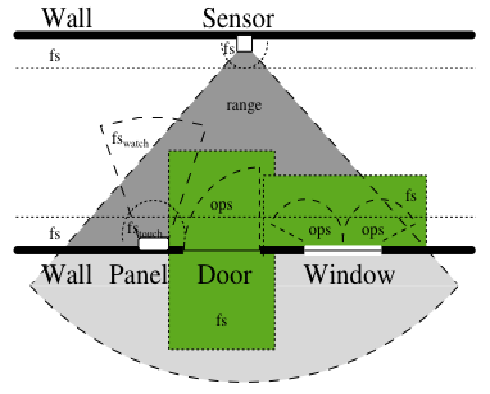
\includegraphics[width=40mm]{functional-space}}
 \hspace{10 mm}
 \subfloat[operational space]{\label{fig:operational-space}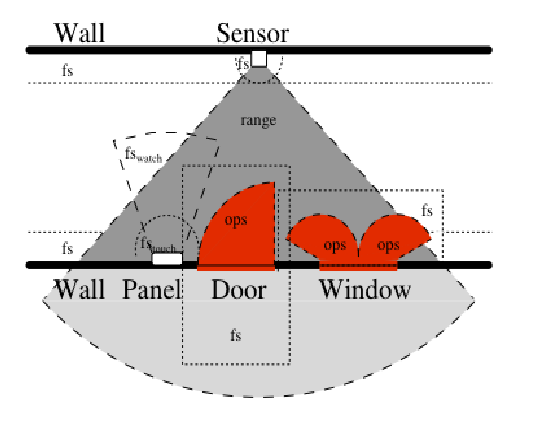
\includegraphics[width=40mm]{operational-space}}
 \hspace{10 mm}
 \subfloat[range space]{\label{fig:range-space}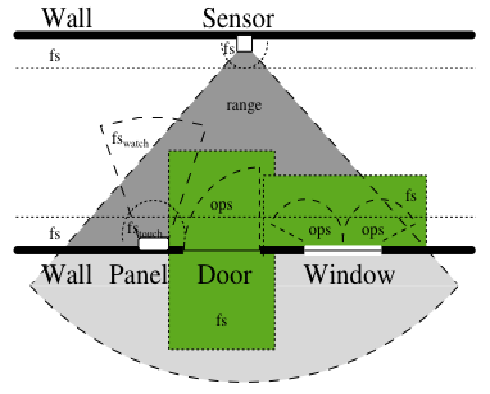
\includegraphics[width=40mm]{functional-space}}
 \caption{Multiple Perspectives}
\label{multi-perspectives}
\end{figure}

Artefactual extensions can effect how a design preforms. For example, a sink in a bathroom has a functional space in-which a person uses the sink to wash his or her hands. If this space is interfered by the functional or physical space of a doorways into the bathroom, then there will be circulation problems when a person is washing their hands and another person enters the bathroom.

TODO: fig:sink example.


\subsubsection{Representation A Design in DSpace}
The representation of a design starts with a factbase in Prolog that links architectural entities (via a unique identifier) to is't architectural type (wall, door, window, column) or interior design type (display case, chair, desk). There is a single entry in the factbase for each entity in the design. The following Prolog code shows one entry for the prototype of the factbase predicate and three instantiated entries for a single door, wall, and desk. 

\begin{verbatim}
   architectural_entity(ID, Type).
   architectural_entity(door1, dSDoor).
   architectural_entity(wall4, dsWallStandardCase).
   architectural_entity(desk4, dsDesk).
\end{verbatim}

Prolog rules are used to link an entity's identifier to its' multiple perspective geometries. Each entity has a single rule for it's physical geometry, and one rule for each of it's artefactual extension: functional space, operational space, range space. Not all entities have all artefactual extension. For example, a door has a functional and operational space but does not have a range space. Likewise, a wall has no artefactual extensions. 

The form of each rule is similar and built using the same spatial primitives (points, lines, and polygons). By using the same spatial primitives to define both the physical structures and aretactual extensions of architectural entities and interior design elements, it allows for a uniform and generalized way to spatial reason over the structures. This will become an important feature in the following section on qualitative spatial reasoning.   

\begin{verbatim}
   physical_geometry(door1, Geometry) :-
           spatial_primitive(Geometry, region(PtList)).
   functional_space(door1, Geometry) :-
           spatial_primitive(Geometry, region(PtList)).
   operational_space(door1, Geometry) :-
           spatial_primitive(Geometry, region(PtList)).
\end{verbatim}

Retrieving a geometry is accomplished in a uniform way across the different perspectives. To get a geometry all that is need is the unique identifier for the entity. For example, to get the physical geometry for a door with and identifier, door1, the following query is made:

\begin{verbatim}
   physical_geometry(door1, Geometry).
\end{verbatim} 
Door1's physical geometry will now by stored in the Geometry variable. Likewise, to get the functional space of door1 the following query is made:
\begin{verbatim}
   functional_geometry(door1, FunctionalGeometry).
\end{verbatim}
Door1's functional geometry will now be stored in the FunctionalGeometry variable. Similar queries are made to retrieve the operational and range space geometries.

\subsection{Spatial Abstraction for Qualitative Spatial Reasoning}
The physical and artefactual geometries in DSpace are generally represented as polygons or extended regions. However, to reason about these spatial structures in a more abstract computational framework, such as a framework for qualitative spatial reasoning, it is required that these architectural entities be spatially abstracted. This means taking into consideration what is meant by the direction of a door, or a wall as a point. How these entities are abstracted will depend on the qualitative spatial reasoning and design requirements that they are meant for. 

For DSpace there are five spatial abstractions that are important: point, directed point, centroid, line, and polygon. The following section on qualitative spatial reasoning will explain why these abstractions are used, for now this section will focus on how the architectural entities in a design are transformed to the various spatial abstractions. 

\subsubsection{Doorways, Windows, and Walls}
Doorways, windows, and walls have point and directed point spatial abstractions. The point abstraction is straightforward and is the centroid of the polygon that makes of the physical geometry of the doorway, window, or wall. The directed point abstraction is the centroid as the origin and the direction is the direction that is perpendicular to the doorway's, window's or wall's intrinsic x-axis. This will give two directions because there will be two perpendicular lines form the origin outwards. This is fine and will actually be useful when reasoning about the direction of a doorways / window in the context of a specific room or area. 

Walls are a special case because the are generally much longer in one axis. TODO: explain this

\subsubsection{Columns}
Columns have only one spatial abstraction which is a point, which is the centroid of the column. Columns do not have any intrinsic qualities which or functional aspects in a design that require any additional abstractions. 

\subsubsection{Spaces: Rooms, Apartments, Buildings}
Spaces such as rooms, apartments, and building can be abstracted as points. The point is the centroid of the space. In general the assumption in DSpace is that spaces are generally rectangular in shape.

\subsubsection{Interior Design Elements}
Interior design elements have two spatial abstractions: point and directed point. The point is the centroid of the element. The directed point must be given by the user for an interior design element because the intrinsic properties of the object can not be known a-priori. If a direction is not provided then an interior design element can not be abstracted into a directed point.

\subsubsection{Spatial Transformations}

\begin{verbatim}
   perspective(id, abstraction, A).
\end{verbatim}

\subsection{IFC / ArchiCAD import}


\section{Spatial Reasoning in a Constraint Logic Programming Framework}
The spatial reasoning module in DSpace is built in a constraint logic programming framework. 

Constraint Handling Rules

Qualification

\subsection{Topology}
Topological reasoning works over points, lines, and regions (convex hulls). The main form of spatial topological reasoning is qualification. The following are the topological relationships that can be qualified: partially overlapping, ntpp, ntppi, disconnected and equals. 

Topological qualifications uses properties of line intersections and convex hulls to detect topological relationships. Constraint handling rules are used to simplify topological constraints until a simple constraint of line intersection checking and point / convex hull containment. The partially overlapping relationship is detected if and lines intersect between objects and 

\subsection{Orientation}

\subsubsection{Intrinsic Orientation}
OPRA
Relationships
  - i, j

Geometric Detection
  - partition of space in to half planes
  - linear inequalities

\subsubsection{Extrinsic Orientation}
SCC
Relationships
  - SCC rel
  
Geometric Detection
  - partition of space into half planes
  - linear inequalities

\subsection{Distance}
Uses Sindalog reasoner's distance constraints
Variation of distance constraints

\subsection{Sample Queries}
Examples with shapes
Examples with architectural elements in the DSpace reasoner


\chapter{Conceptual Design Requirements}
This chapter presents a hierarchical structure for building conceptual design requirements, demonstrates how the elements that build conceptual design requirements can be spatially interpreted in the context of formal qualitative spatial calculi, and used to validate design requirements in the computational framework of the DSpace reasoner. 

Conceptual design requirements, and the elements used to build them (architectural concepts and qualitative spatial attributes found in architecture) were ascertained from literature on architectural design \cite{tbd}, museum research on visitor behavior \cite{tbd}, and building regulations and codes \cite{tbd}. Their definitions are explicit characterizations of architectural concepts and design qualities that are based on heuristic architectural knowledge and common sense notions of spatial relationships. The objective is not to be an exhaustive discussion of these requirements or a validation for their interpretation in terms of a spatial or design perspective; rather it is to demonstrate how each can be represented and reasoned with in a computational framework to validate conceptual design requirements against the quantitative structures and artifacts of a design. 

The chapter is structured as follows: Section 1 describes the hierarchical structure of conceptual design requirements. Section 2 presents a set of qualitative spatial attributes found in architecture, shows how each can be interpreted using formal qualitative spatial calculi, and represented formally within DSpace reasoner. Section 3 presents a set of architectural concepts that are built using the spatial qualities presented in the section 2 and shows how they can be used to reason about design requirements within the DSpace reasoner. Section 4 demonstrates how a the DSpace reasoner can be used to validate a design per it's conceptual design requirements.

\section{Hierarchy}
The design hierarchy developed in this section is built on the discretion of the design problem into a design space, a quality space, and a quantity space. At the highest level, the design space involves the architectural design semantics (architectural concepts) and qualities (qualitative spatial attributes found in architecture) that emerge in architecture. At the lowest level, the quantitative space involves the precise geometries of the architectural structures found in the design. The qualitative space mediates between the abstractions of the design layer and the concreteness of the quantitative later using qualitative spatial representation and reasoning.
 
\begin{figure}[H]
\centering

\includegraphics[width=140mm]{hierarchy2}
\caption{Design Space Hierarchy}
\label{hierarchy}
\end{figure}

Figure \ref{hierarchy} shows the design hierarchy used in the DSpace reasoner. Conceptual design requirements are built from the architectural concepts and QSA's of the hightest level of the hierarchy. Within the hierarchy, architectural concepts are built using qualitative spatial attributes found in architecture (QSA), but are not limited to only these, spatial relationships of orientation, topology, and distance can be used, as well as other geometric primitives such as area, angle, and length measurements. QSAs are defined by the qualitative spatial relationships of orientation, topology, and distance. These qualitative spatial relationships emerge from the quantitative, physical, and artefactual geometries of the the design. TBD: physical structures define the way the architecture is experiences and influences the functional / performance of the design from a conceptual design perspective.


\section{Qualitative Spatial Attributes found in Architecture}
This section presents a set of qualitative spatial attributes found in architecture (QSA) and shows how each QSA is spatially interpreted and represented in DSpace. QSAs are architectural qualities that emerge from the spatial structures that form from the physical elements of the building (doors, walls, columns, windows, etc.), artefactual extensions (functional space, operational space, range space, etc.) and interior design elements (furniture, lights, decorations, etc.). QSAs can be perceptual qualities that are described from a specific vantage point, or intrinsic qualities that are inherent in the build's spatial structure. 

This section presents five QSAs: positioning, facing, visibility, proximity, and symmetry. The goal of this section is to develop a tool-kit of QSAs that qualitatively describe architectural designs in the spatial environments in which they emerge. Some boundary cases are identified and handled, but it is not the purpose here to explore all possible case scenarios.

\subsection{Positioning}
The positioning attribute defines an orientational relationship between a pair of objects as each object relates to the other within an extrinsic context, i.e., a defined space such as a room, apartment, building, or user defined space. There are four positioning relationships using this scheme: opposing-side of space, same-side of space, left-side of space, and right-side of space. The opposing-side and same-side relationships can be combined, via conjunction, with the left-side or right-side relationships to form the following compound relationships: opposing-left-side, opposing-right-side, same-left-side, same-right-side.

\begin{figure}[H]
\centering
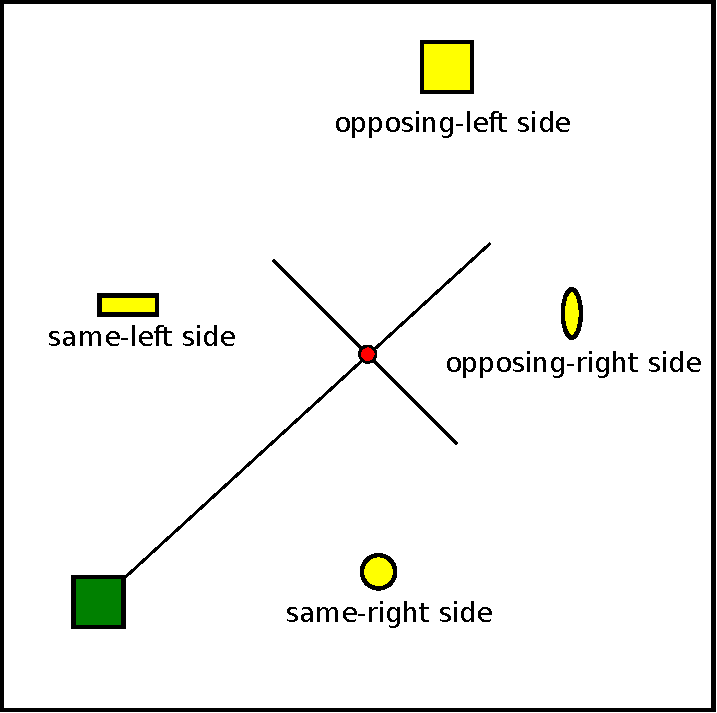
\includegraphics[width=80mm]{position}
\caption{Positioning}
\label{position}
\end{figure}

The positioning attribute is interpreted spatially, in DSpace, using the Single Cross (SCC) orientation calculus \cite{Freksa92usingorientation}. SCC defines the orientation of a point C (referent) with respect to a point B (relatum) from the viewpoint of a point A (origin). The positioning attribute uses the SCC partitioning scheme to orientationally relate two points (origin, referent) in the context of an external frame of reference (relatum). In DSpace, the reference point is defined as the centroid of the context space. By partitioning space using the centroid, an approximation is made that divides the space into the positioning relationships. An assumption made in DSpace is that the space will generally be rectangular in shape.

\begin{figure}[H]
\centering
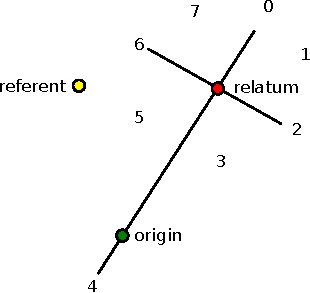
\includegraphics[width=60mm]{scc}
\caption{SCC Partitioning}
\label{scc}
\end{figure}

Under this scheme, two points are defined as being on opposing sides of a space if they have an SCC relationship of 0, 1 or 7, as related by the centroid of the space. Conversely, a pair of points are defined as being on the same side of a space if they have an SCC relationship of 3, 4 or 5, as related by the centroid of the  space. A point is defined as being on the left side of a space from another point if it has an SCC relationship of 1, 2, or 3, and is on the right side if it has an SCC relationship of 5, 6, or 7. Using the union set operation these relationships can be combined to form the opposing-left/right, and same-left/right relationships.

Th positioning relationships are represented in DSpace as Prolog rules. There is a single rule for each relationships: opposing side, same-side, left-side, and right-side. The head of each rule takes three arguments, the first two for the architectural objects being related and one for the context space. The body of the rule .... Given two objects and a context space, the rule returns true if the objects are on the same-side, opposing-side, left-side, right-side as defined by its' rule, and fails if they are not. The following is Prolog code for the positioning rules.

\begin{verbatim}
   opposing_side(Obj1, Obj2, Context) :- 
           centroid(Context, Centroid),
           (scc(Obj1, Centroid, Obj2, 0);
            scc(Obj1, Centroid, Obj2, 1);
            scc(Obj1, Centroid, Obj2, 7)).
                                          
   same_side(Obj1, Obj2, Context) :- 
           centroid(Context, Centroid),
           (scc(Obj1, Centroid, Obj2, 2) ;
            scc(Obj1, Centroid, Obj2, 3) ;
            scc(Obj1, Centroid, Obj2, 4) ;
            scc(Obj1, Centroid, Obj2, 5) ;
            scc(Obj1, Centroid, Obj2) 6)).   

\end{verbatim}

The positioning attribute can be used to check if architectural structures, artefactual extensions, or interior design elements are on the opposing or same side of a space to the other. For example, a requirement might state that a bedroom should be positioned to the back of a house from the main entrance. The reason for this requirement is that rooms that are in the back of a house are more private than rooms in the front of the house. In this requirement, the origin is the entrance, the referent is the bedroom, and the relatum is the centroid of the house (context space).

\begin{figure}[H]
 \centering
 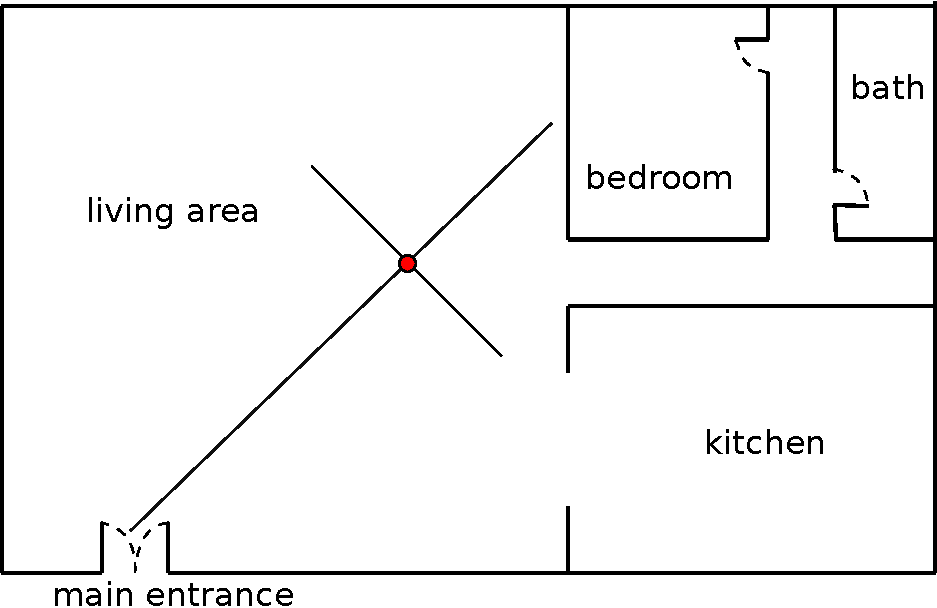
\includegraphics[width=95mm]{bedroom-back-house}
 \caption{Bedroom Privacy}
\label{privacy}
\end{figure}


\subsection{Facing}
The facing attribute defines an intrinsic orientational relationship between two objects as each object relates to the other. The definition used here is based on a common sense interpretation of facing, in which an object \emph{A} is facing towards an object \emph{B}, if \emph{B} is in front of \emph{A} and \emph{A} is directionally oriented at \emph{B}. Under this definition, a pair of objects can be facing towards or away from each other. Given a pair of objects, \emph{A} and \emph{B}, there are four possible facing configurations between the pair: 

\begin{figure}[H]
 \centering
 \subfloat[A, B towards]{\label{fig:facing-towards}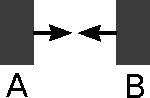
\includegraphics[width=25mm]{facing-towards}}
 \hspace{10 mm}
 \subfloat[A, B away]{\label{fig:facing-away}
\includegraphics[width=28mm]{facing-ABaway}}
  \hspace{10 mm}
 \subfloat[A towards, B away]{\label{fig:facing-A}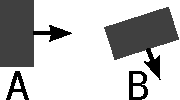
\includegraphics[width=28mm]{facing-Atowards-Baway}}
 \hspace{10 mm}
 \subfloat[A away, B towards]{\label{fig:facing-A}
\includegraphics[width=28mm]{facing-Aaway-Btowards}}
 \caption{facing}
\label{display-arrangement}
\end{figure}

The facing attribute is spatially modelled in DSpace using the Oriented Point Relation Algebra \cite{Moratz} (OPRA). The advantage of using OPRA is that it models the intrinsic orientational relationships between a pair of directed points. OPRA partitions space into half planes, which are defined by lines emanating outwards from the reference point, and defines the qualitative orientational relationships by the half plane in which a second point is located. The granularity of an OPRA relationships is defined by the number of lines emanating from the point. 

Figure \ref{facing-opra-base-rel} shows the OPRA$_{2}$ (two lines) partitioning of space, with labels for the base relationships. Point \emph{A} is located in sector 7 of point \emph{B}'s partitioned space, and \emph{B} is located in sector 1 of \emph{A}'s partitioned space. Note that the arrow depicts the point's direction and the half-plane sectors are labelled starting at the point's direction, incrementing counter-clockwise. 

\begin{figure}[H]
\centering

\includegraphics[width=60mm]{facing-opra-base-rel}
\caption{OPRA$_{2}$ Space Partitioning}
\label{facing-opra-base-rel}
\end{figure}

Using OPRA$_{8}$, the facing attribute can be defined in terms of the half plane sectors. Point \emph{A} is facing towards point \emph{B}, if \emph{B} is located in sectors 0, 1, or 32 of \emph{A}'s partitioned space. Similarly, if \emph{A} is located in sectors 0, 1, or 32 of \emph{B}'s partitioned space then \emph{B} is facing towards \emph{A}. In this case, both points are facing towards each other. Conversely, point \emph{A} is facing away from point \emph{B} if \emph{B} is located in sectors 2 - 31 of \emph{A's} partitioned space. An OPRA 8 granularity is used to define a narrow interpretation of the facing attribute. Within a room, doorways, windows, and walls are generally face towards each other. By narrowing the space that is considered facing towards, it allows DSpace to detect elements that are more directly facing towards each other.

Figure \ref{fig:facing-opra-towards} shows an example of two points facing towards each other; note that each point is located in sector 32 of the other's partitioned space.  Figure \ref{fig:facing-opra-away} shows an example of two points that are facing away from each other and are not located in sectors 0, 1, 32 of the other's partitioned space. 

\begin{figure}[H]
 \centering
 \fbox{
 \subfloat[facing towards]{\label{fig:facing-opra-towards}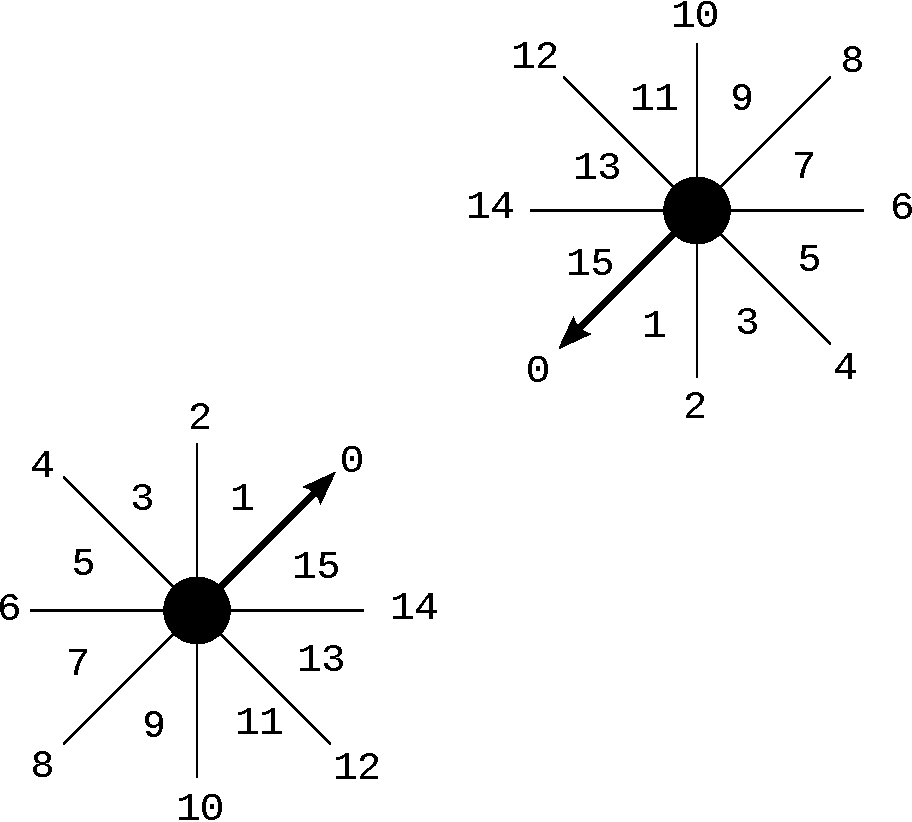
\includegraphics[width=60mm]{facing-opra}}
 }
  \hspace{10 mm}
  \fbox{
 \subfloat[facing away]{\label{fig:facing-opra-away}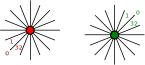
\includegraphics[width=60mm]{facing-away-opra}}
 }
 \caption{OPRA Partitioning }
\label{opra-facing}
\end{figure}

The facing attribute is represented in DSpace as Prolog rules. There is one rule for facing-towards and one for facing-away. The head of each rule takes two arguments for the objects being related. The body of the rule is a single disjunctive clause that checks for the OPRA$_{8}$ relationship between the objects. Given two objects, the rule returns true if the objects are facing towards or away from each other as defined by the rule, and fails if they are not. The following is Prolog code for the facing rules.

\begin{verbatim}
   facing_towards(Obj1, Obj2) :- 
           (opra(Obj1, Obj2, 0) ;
            opra(Obj1, Obj2, 1) ;
            opra(Obj1, Obj2, 32)).
                                 
   facing_away(Obj1, Obj2) :- 
           not facing_towards(Obj1, Obj2).                     
\end{verbatim}

In DSpace, the facing attribute can be used to check if two architectural structures, artefactual extensions, or interior design elements are facing towards or away from each other. For example, doorways and windows that face towards each other promote airflow through the space they inhibit. A design that requires good air circulation could use this knowledge to ensure proper airflow. Figure \ref{door-window-facing} shows two example floor plans of a room with a window and doorway. Figure \ref{fig:door-window-towards} shows a configuration were the doorway and window are facing towards each other, while figure \ref{fig:door-window-away} shows a configuration where the doorway and window are facing away from each other. 

\begin{figure}[H]
 \centering
 \subfloat[facing towards]{\label{fig:door-window-towards}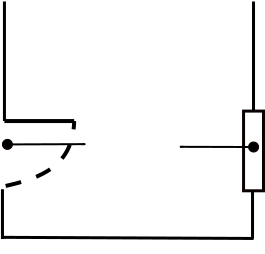
\includegraphics[width=55mm]{door-facing-window-con}}
  \hspace{10 mm}
 \subfloat[facing away]{\label{fig:door-window-away}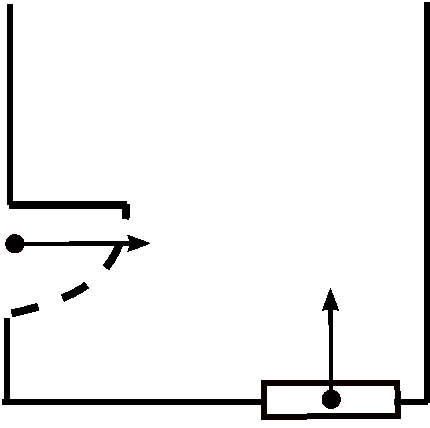
\includegraphics[width=53mm]{door-facing-window-incon}}
 \caption{Door, Window Facing}
\label{door-window-facing}
\end{figure}

TBD: example, operational space of information kiosk should face towards the entrance.

Within the context of architecture, care needs to be taken to account for architectural structures that are long in one axis, such as walls, because the spatial abstraction for OPRA is a directed point. This means that an object is defined as facing towards a wall if it is facing towards the wall's directed point abstraction (usually the centroid of the wall). Under this definition, there are configurations where an object should be considered to be facing a wall but it is not. DSpace handles this special case by modifying the OPRA$_{8}$ relationships that correspond to facing towards and away from a wall. 

fig: wall example

\subsection{Proximity / Distance}
The proximity attribute defines a qualitative distance relationship between two objects. In DSpace, there are three proximity relationships: near, near+, and far. The spatial interpretation of proximity depends on the context and scale which the objects inhibit. In the context and scale of architectural space, proximity is defined using heuristics based on the scale of building elements, i.e. rooms, apartments, buildings.

\begin{figure}[H]
\centering
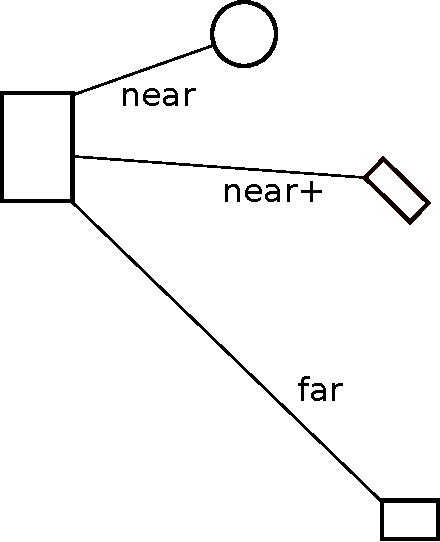
\includegraphics[width=45mm]{proximity}
\caption{Proximity}
\label{proximity}
\end{figure}

Using these heuristics, two objects are near if the minimum distance between them is less then or equal to 3 meters, near+ if the minimum distance between then is between 3 - 6 meters, and far if the minimum distance between them is greater then 3 meters. While the definition of proximity pivots around 3 and 6 meters, it can easily be changed by using an extra parameter in a proximity predicate. 

Proximity is represented in DSpace as three Prolog rules. There is one rule for near, one for near+, and one for far. The head of each rule takes two arguments for the architectural objects being related. The body of the rule .... Given two objects, the rule returns true if the objects are near, near+, or far from each other as defined by the rule, and fails if they are not. The following is Prolog code for the proximity rules.

\begin{verbatim}
   near(Obj1, Obj2) :- 
           minimum_distance_compare(Obj1, Obj2, <=, 3).
   
   near_plus(Obj1, Obj2) :-
           minimum_distance_compare(Obj1, Obj2, <=, 6),
           minimum_distance_compare(Obj1, Obj2, >, 3).   
   
   far(Obj1, Obj2) :- 
           minimum_distance_compare(Obj1, Obj2, >, 6)

\end{verbatim}

The proximity attribute can be used to check whether two architectural structures, artefactual extension, or interior design elements are near or far. For example, a computer desk should be located near a power outlet to make it easy to power up the desk's computer and desk's lamp. Another example is the bathroom should be far away from the kitchen, in order to keep a separation between the two.

\begin{figure}[H]
 \centering
 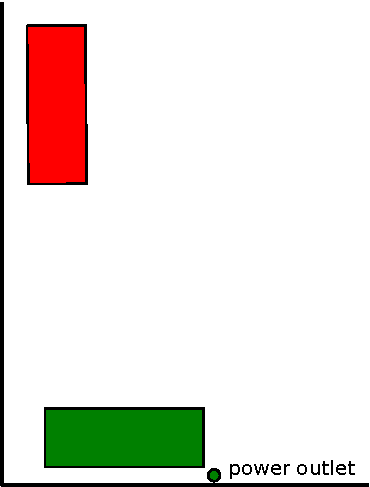
\includegraphics[width=50mm]{desk-proximity}
 \caption{Desk Outlet Proximity}
\label{desk-proximity}
\end{figure}

\subsection{Visibility}
The visibility attribute defines a boolean relationship between a viewpoint and an object with respect to the object being visible from the viewpoint. An objects is visible if the view-space (i.e., the space between the viewpoint and the object) is not obstructed. This definition of visibility does not take into account the effects of distance on visibility, i.e., an object that is very far away is not visible. However, within the context of architecture and buildings, the magnitude of distances is limited to a point that it is not a factor to visibility.

The spatial interpretation of visibility is based on the topological characteristics of the space in-between the viewpoint and object. This space is referred to as the view-space. An object is visible if the view-space is not obstructed by surrounding structures or objects. An obstructing object is an object that has a partially overlapping or containing topological relationship with the view-space. Artefactual extension is not considered as an obstructing object because it does not have a physical form. This definition does not distinguish between visibility that is partially or totally obstructed.

\begin{figure}[H]
 \centering
 \subfloat[obstructed view]{\label{fig:obstructed-view}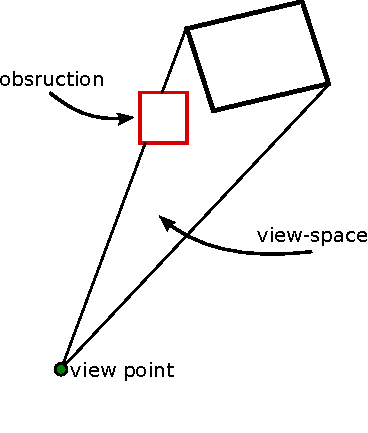
\includegraphics[width=55mm]{visibility}}
  \hspace{10 mm}
 \subfloat[non-obstructed view]{\label{fig:no-obstruction}
\includegraphics[width=55mm]{visibility-no-obstruction}}
 \caption{Visibility}
\label{Visibility}
\end{figure}



Visibility is represented in DSpace as a single Prolog rule. The head of the rule takes two arguments, the viewpoint and the object that is being check for visibility. The body of the clause calculates the view-space and checks the surrounding objects for a topological obstruction. Given a viewpoint and an object, the rule returns true if the object is visible, and fails if it is not. The following is the Prolog code for the visibility rule.

\begin{verbatim}
   is_visible(ViewPoint, Obj) :- 
           view_space(ViewPoint, Obj, ViewSpace),
           topology(ViewSpace, SurroundingStructs).
\end{verbatim}

The visibility attribute can be used to check if an architectural structure or interior design element is visible from a given viewpoint. For example, an architect might want to ensure that a staircase is visible from the main entrance of a building, because she doesn't want the staircase to go unnoticed. Figure \ref{visibility-door-stair} shows and example floor plan where the stairway is not visible from the doorway. In this example both the wall in red and column are obstructing the view from the doorway. 

\begin{figure}[H]
\centering
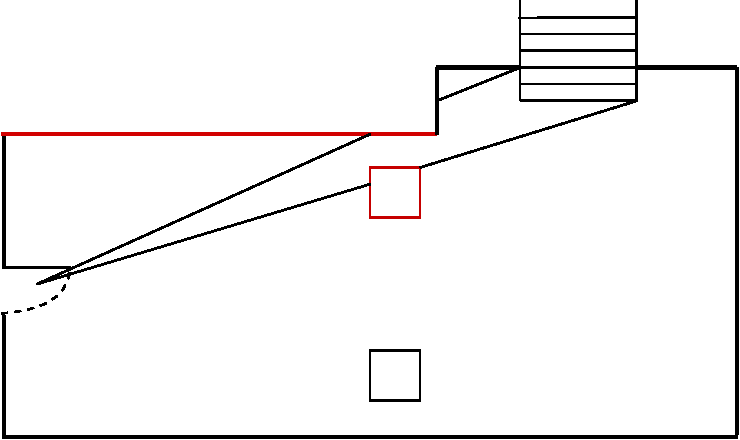
\includegraphics[width=80mm]{visibility-stair-door}
\caption{Visibility Example: Doorway and Stairs}
\label{visibility-door-stair}
\end{figure}

\subsection{Alignment / Symmetry}

TBD: I have a loose idea about this property but the idea needs more development

\subsection{Pathways / Turns}  right turn (hard) / left turn (hard) / straight 

TBD: I have a loose idea about this property but the idea needs more development

\section{Architectural Concepts}
Architectural concepts, such as privacy, continuity, and enclosure, describe an experiential aspect of architecture as used by an architect to describe the functionality of a design \cite{Koile}. These terms are defined in DSpace in a hierarchical manner in which architectural concepts are built using QSAs and geometric primitives (orientation, topology, distance). 

This section presents four architectural concepts and demonstrates how each is defined in DSpace. As in the previous section, the purpose is not to investigate the correctness of the concepts or an attempt to compile a complete list, rather it is to look at how these concepts can be defined logically using architectural qualities and spatial / geometric primitives.

\subsection{Privacy}
In architecture, the concept of privacy implies a notion of separation and obscurity (not being visible). In the case of a room, privacy can be defined as being separated from the main entrance of the building and having doorways that enhances the room's privacy. A doorway can be be defined as private with respect to its functionality of connecting two adjacent areas (rooms, hallways, etc.). Under this consideration, a doorway can enhance or hinder the privacy of a room. A doorway enhances privacy of a room if the doorway faces away from other local doorways (doorways in adjacent rooms) and if it is not visible from the main living space. 

Within DSpace, the concepts of privacy has been formally defined for rooms and doorways. A door is private if it has the following attributes: (1) it is not visible from the main living space, (2) it does not mutually face towards another doorway and (3) it does not face towards the centroid of an adjacent room. A room is private if it has the following attributes: (1) it is positioned on the opposing side of the building with regard to the main entrance and (2) all doorways into the room are private, per the doorway privacy definition.
 
Privacy is represented in DSpace as Prolog rules. The rules take a single argument, in the head, which indicates if the rule is for a room or doorway. The body of the rule defines the properties of the privacy using QSAs, as defined above. Note that there are two predicates, one for the definition of privacy for a room and one for privacy of a doorway.  

\begin{verbatim}
   private(room) :-  
           opposing_side(room, main_entrance, building), 
           private(doorway).
                     
   private(door) :- 
           facing_away(door, door),
           facing_away(door, adjacent_space),
           not_visible(door, main_living_space). 
\end{verbatim}

Figure \ref{room-privacy} shows two floor plans for a small single bedroom house; figure \ref{fig:private-room-con} shows a floor plan with a bedroom that is  private, while figure \ref{fig:private-room-incon} shows a similar floor plan with a bedroom that is not private. The numbers in the figures represent the following privacy requirements: (1) the bedroom is positioned on the opposing side of the building with regards to the main entrance, (2) the doorway is not visible from the main living space, and (3) the doorway does not mutually face towards another doorway. Numbers that are colored red indicate that the requirement has been broken, while numbers in green indicate that the requirement has been met.

\begin{figure}[H]
 \centering
 \subfloat[Private]{\label{fig:private-room-con}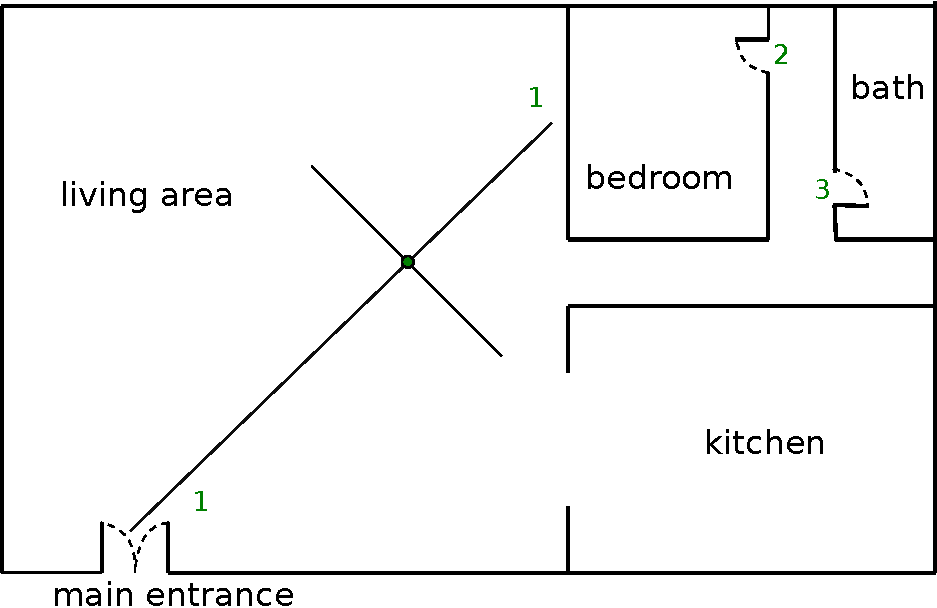
\includegraphics[width=69mm]{privacy-room-con}}
  \hspace{5mm}
 \subfloat[Not Private]{\label{fig:private-room-incon}
\includegraphics[width=69mm]{privacy-room-incon}}
 \caption{Bedroom Privacy}
\label{room-privacy}
\end{figure}

\subsection{Continuity}
In architecture, the concept of continuity describes a network of points that are mutually visible \cite{Key}. In DSpace, continuity is interpreted in the context of building navigation and wayfinding. Under this interpretation, a building, room or apartment is continuous if there is continuity between the doorways contained in a given space: room, building, or apartment. 

Continuity is defined as a network of doorways that are mutually visible. The partitioning of doorways that should be mutually visible is based on a localized containment hierarchy between rooms and doorways, in which doorways that are contained in the same room should maintain continuity. It does not make sense for doorways that are located on opposite sides of a building to be visible to each other, but doorways that are in the same room should be. 

With respect to this definition, continuity is represented as a recursive rule in Prolog, which takes a list of doorways and checks that each doorway is mutually visible to the others within the list. (need to mention doorways within a room). TBD: arguments: list of doors or room id that indicates containment level???

\begin{verbatim}
   continuous([Obj1,Obj2|[]]) :- 
           is_visible(Obj1, Obj2).

   continuous([Obj1,Obj2|OS]) :- 
           is_visible(Obj1, Obj2),
	       is_visible(Obj2, Obj1),
           continuity([Obj1|OS]),
           continuity([Obj2|OS]).
\end{verbatim}

Figure \ref{continuity} shows a floor plan for a single room with three doors. Figure \ref{fig:continuity-con} shows a configuration in which each door is mutually visible to the other doors. This design is continuous. Conversely, figure \ref{fig:continuity-incon} shows a configuration in which door 1 is not mutually visible to door 2 and door 1 is not mutually visible door 3. The visibility between door 1 and door 2 is obstructed by a column and the visibility between door 1 and door 3 is obstructed by a wall. Structural elements that are colored red indicated a visibility obstruction. This design is not continuous. 

\begin{figure}[H]
 \centering
 \subfloat[Consistent]{\label{fig:continuity-con}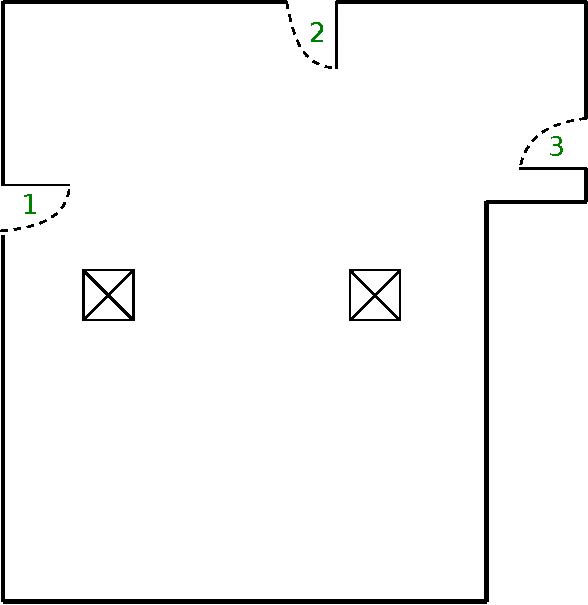
\includegraphics[width=45mm]{continuity-con}}
  \hspace{30 mm}
 \subfloat[Inconsistent]{\label{fig:continuity-incon}\includegraphics[width=45mm]{continuity-incon}}
 \caption{Continuity}
\label{continuity}
\end{figure}

\subsection{Enclosure} 
In architecture, the concept of enclosure defines a space, as experienced from a given vantage point, as being confined or open. A confined space is defined as being confined by walls or columns, while an open space is defined as being spacious. In DSpace, enclosure is defined by localized spatial structures in terms of their proximity to a given point. Under this interpretation, a room, apartment, or building can be experienced as both confined and open based on the location of the vantage point within the space. Such a definition takes into account that enclosure is locally experienced. For example, an alcove in an otherwise open room, feels confined when experienced from inside the alcove.

In Dspace, a point is defined as open if less then three walls or columns are near-to the point. Conversely, a point is defined as confined if three or more walls or columns are near-to the point. While this interpretation of enclosure is naive, it maintains the notion that proximity defines the spatial structures of openness and confinement in a localized environment.   

\begin{verbatim}
confined(point) :-  

spacious(point) :-

\end{verbatim} 

Figure \ref{enclosure} shows a floor plan for a single room with various enclosure properties. The room contains an alcove and a sequence of columns that will provide an environment of confinement. Points in-between the columns and inside the alcove are confined because of the proximity of the walls and/or columns. The points outside of these areas are open because there are few structures nearby.

\begin{figure}[H]
\centering
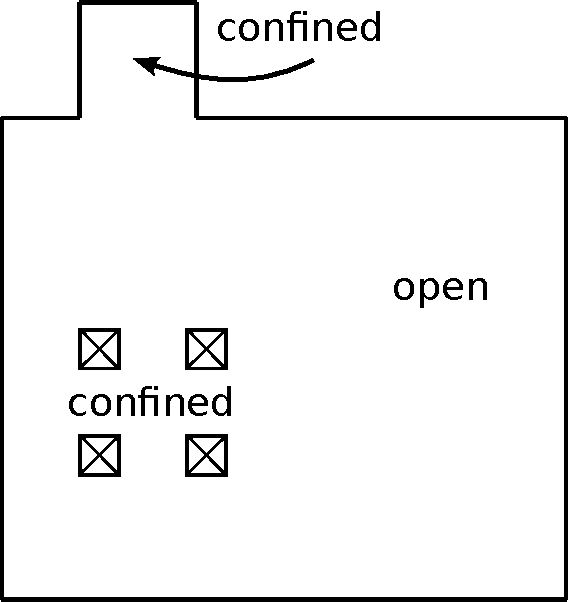
\includegraphics[width=60mm]{spacious-confined}
\caption{Enclosure, Confined and Open}
\label{enclosure}
\end{figure}


\subsection{Building Regulations and Codes}
Building regulations and codes are a special case in this section because they are not strictly architectural concepts. However, they provide a unique set of architectural requirements that incorporate a breadth of design aspects. This section will take a look at two such requirements: building surveillance and artefactual interference. These requirements were picked specifically because each incorporate artefactual aspects of the design problem. 

\subsubsection{Artefactual Interference}
Artefactual interference deals with the unintentional interactions of the operational and functional spaces of a building's structural form. For example, the operational space of a bathroom doorway that overlaps with the functional space of the bathroom sink will cause circulation problems into and out of the bathroom. In DSpace, this type of interaction can be detected using topological reasoning over the artefactual extensions of the entities. 

TBD: fig:sink example

This type of artefactual interaction can be checked for in DSpace using a single rule that takes two arguments in the head of the rule. The body of the rule retrieves the artefactual geometry of each element and checks their topological relationship. It fails if the artefacts have an overlapping relationship.

\begin{verbatim}
   bathroom_sink_door(sink, door) :- 
           artefact_geometry(sink, Artefact_sink),
           artefact_geometry(door, Artefact_door),
           not_overlapping(Artefact_sink, Artefact_door).
\end{verbatim}

Artefactual interactions can be between a physical structure (door, wall, column, ect.) and artefactual extension. For example, the landing space (operational space in DSpace parlance) of a stair should be clear. Representing this requirement is similar to the bathroom sink example except that it checks for interactions between the stair's artefactual space with the building physical space.

In DSpace this can be represented as a single rule. The body of the rule checks for an overlapping relationship between the landing space of the stair and both the artefactual extension and physical structure of surrounding elements.

TBD: figure of stair landing

\begin{verbatim}
    clear_stair_landing(stair, Obj) :- 
            artefact_geometry(stair, Artefact_stair),
            artefact_geometry(Obj, Artefact_obj),
            physical_geometry(Obj, Physical),
            not_overlapping(Artefact_stair, Artefact_obj),
            not_overlapping(Artefact_stair, Physical)
\end{verbatim}  

\subsubsection{Surveillance}
Surveillance involves the placement of cameras within a building to provide security. A well functioning surveillance system has specific spatial properties with regard to the placement of the cameras to the structures they survey. For example, a surveillance system could monitor activity at doorways. In this situation the spatial relationships between the camera, its range space (i.e., the camera's surveillance area) and the doorways are important. Such a requirement could be expressed as the functional space of every doorway should overlap with the range space of at least one camera. 

\section{Using The DSpace Reasoner}

This section will describe how to use the DSpace reasoner from a practical perspective....

\chapter{Museum Case Study}
This chapter is a case study that demonstrates the application of the DSpace reasoner to the design of an art museum. The purpose is twofold: first, to examine several design requirements of an art museum with regards to the spatial interpretation of the requirements; and second, to show how the museum design requirements can be represented and reasoned about in a computational framework, in order to detect design inconsistencies as per the design requirements.

The remainder of the chapter is divided into three sections. The first section examines design requirements in art museums in three parts: the first part looks at requirements that influence museum visitors' behaviour. The second part looks at requirements for promoting exploration in the museum. The third part looks at the requirements of accessibility and security within the museum. The second section, looks at how these requirements can be interpreted spatially and represented in the DSpace reasoner. The third section tests the DSpace reasoner using sample museum floor plans that are both consistent and inconsistent per the design requirements for several art museums. The objective of this demonstration is to show that the DSpace reasoner can validate a design against its design requirements.


\section{Case Study Scenario: an art museum}
Museums are a place of public education, in which art, historical artefacts, and scientific exhibits are put on display for the public to view \cite{Falk}. While museums in general have many common threads in terms of their design requirements, this case study takes the approach of narrowing the study to that of an art museum. This focuses the discussion to specific real world examples and maintains the perspective that this is not an exhaustive study of museum design requirements, rather it's an investigation into the nature and interpretation, with respect to spatial properties / characteristics, of a set of design requirements. Additionally, the point is not to prove the validity of these requirements in an empirical sense; rather it is to show the process of representing and reasoning about design requirements in a formal computational framework.

The art museum is a unique and fruitful choice for this case study because it provides a rich set of design properties that have been formally studied and reported \cite{Melton} \cite{Bitgood02} \cite{Falk}. Within museum studies, visitor behaviour has been one of the primary focuses, starting with experiments dating back to the 1930's. 



\subsection{Museum Design Requirements}
Pretend for a moment that you are an architect working on the initial design for a new modern art museum. During your first visit with the museum's curator you discuss several design requirements that are important for the new museum. Your discussion reveals that the curator wants the new art museum to adhere to the following requirements:

\begin{enumerate}
\item Maximize visitor utilization of exhibitions
\item Encourage free-flowing exploration throughout the museum
\item Adhere to museum requirements of accessibility and security
\end{enumerate}

TBD: explain how these high level requirements can be interpreted into concrete properties of the museums design. from here the requirements can be spatially interpreted and represented in the DSpace reasoner.

\subsection{Maximizing Visitor Utilization of Exhibitions}
This portion of the case study will look into four factors that influence visitors' movement patters: positioning of doorways, spatial arrangement of display cases, positioning of furniture and statues, and congestion. These properties inform museum architects, during the design process, about the spatial characteristics that can maximize the utilization of the museum by increasing the frequency and duration with which visitors view exhibition objects. 

\subsubsection{Positioning of doorways}
In an important study, Melton \cite{Melton} discovered that the most influential factor to determine  the amount of attention an object receives is the object's position relative to doorways in a gallery room. Prior to this, museum researchers believed that the object's intrinsic properties of 'interestingness', color, and size were the real factors that determined the amount of attention an object received. Melton explained why this happens; he demonstrated that the amount of attention an object receives is directly related to the visitor circulation patterns within the museum and these circulation patterns emerge from the spatial characteristics of the museum's architecture.

\begin{figure}[H]
 \centering
 \subfloat[circulation pattern]{\label{fig:door-opposite}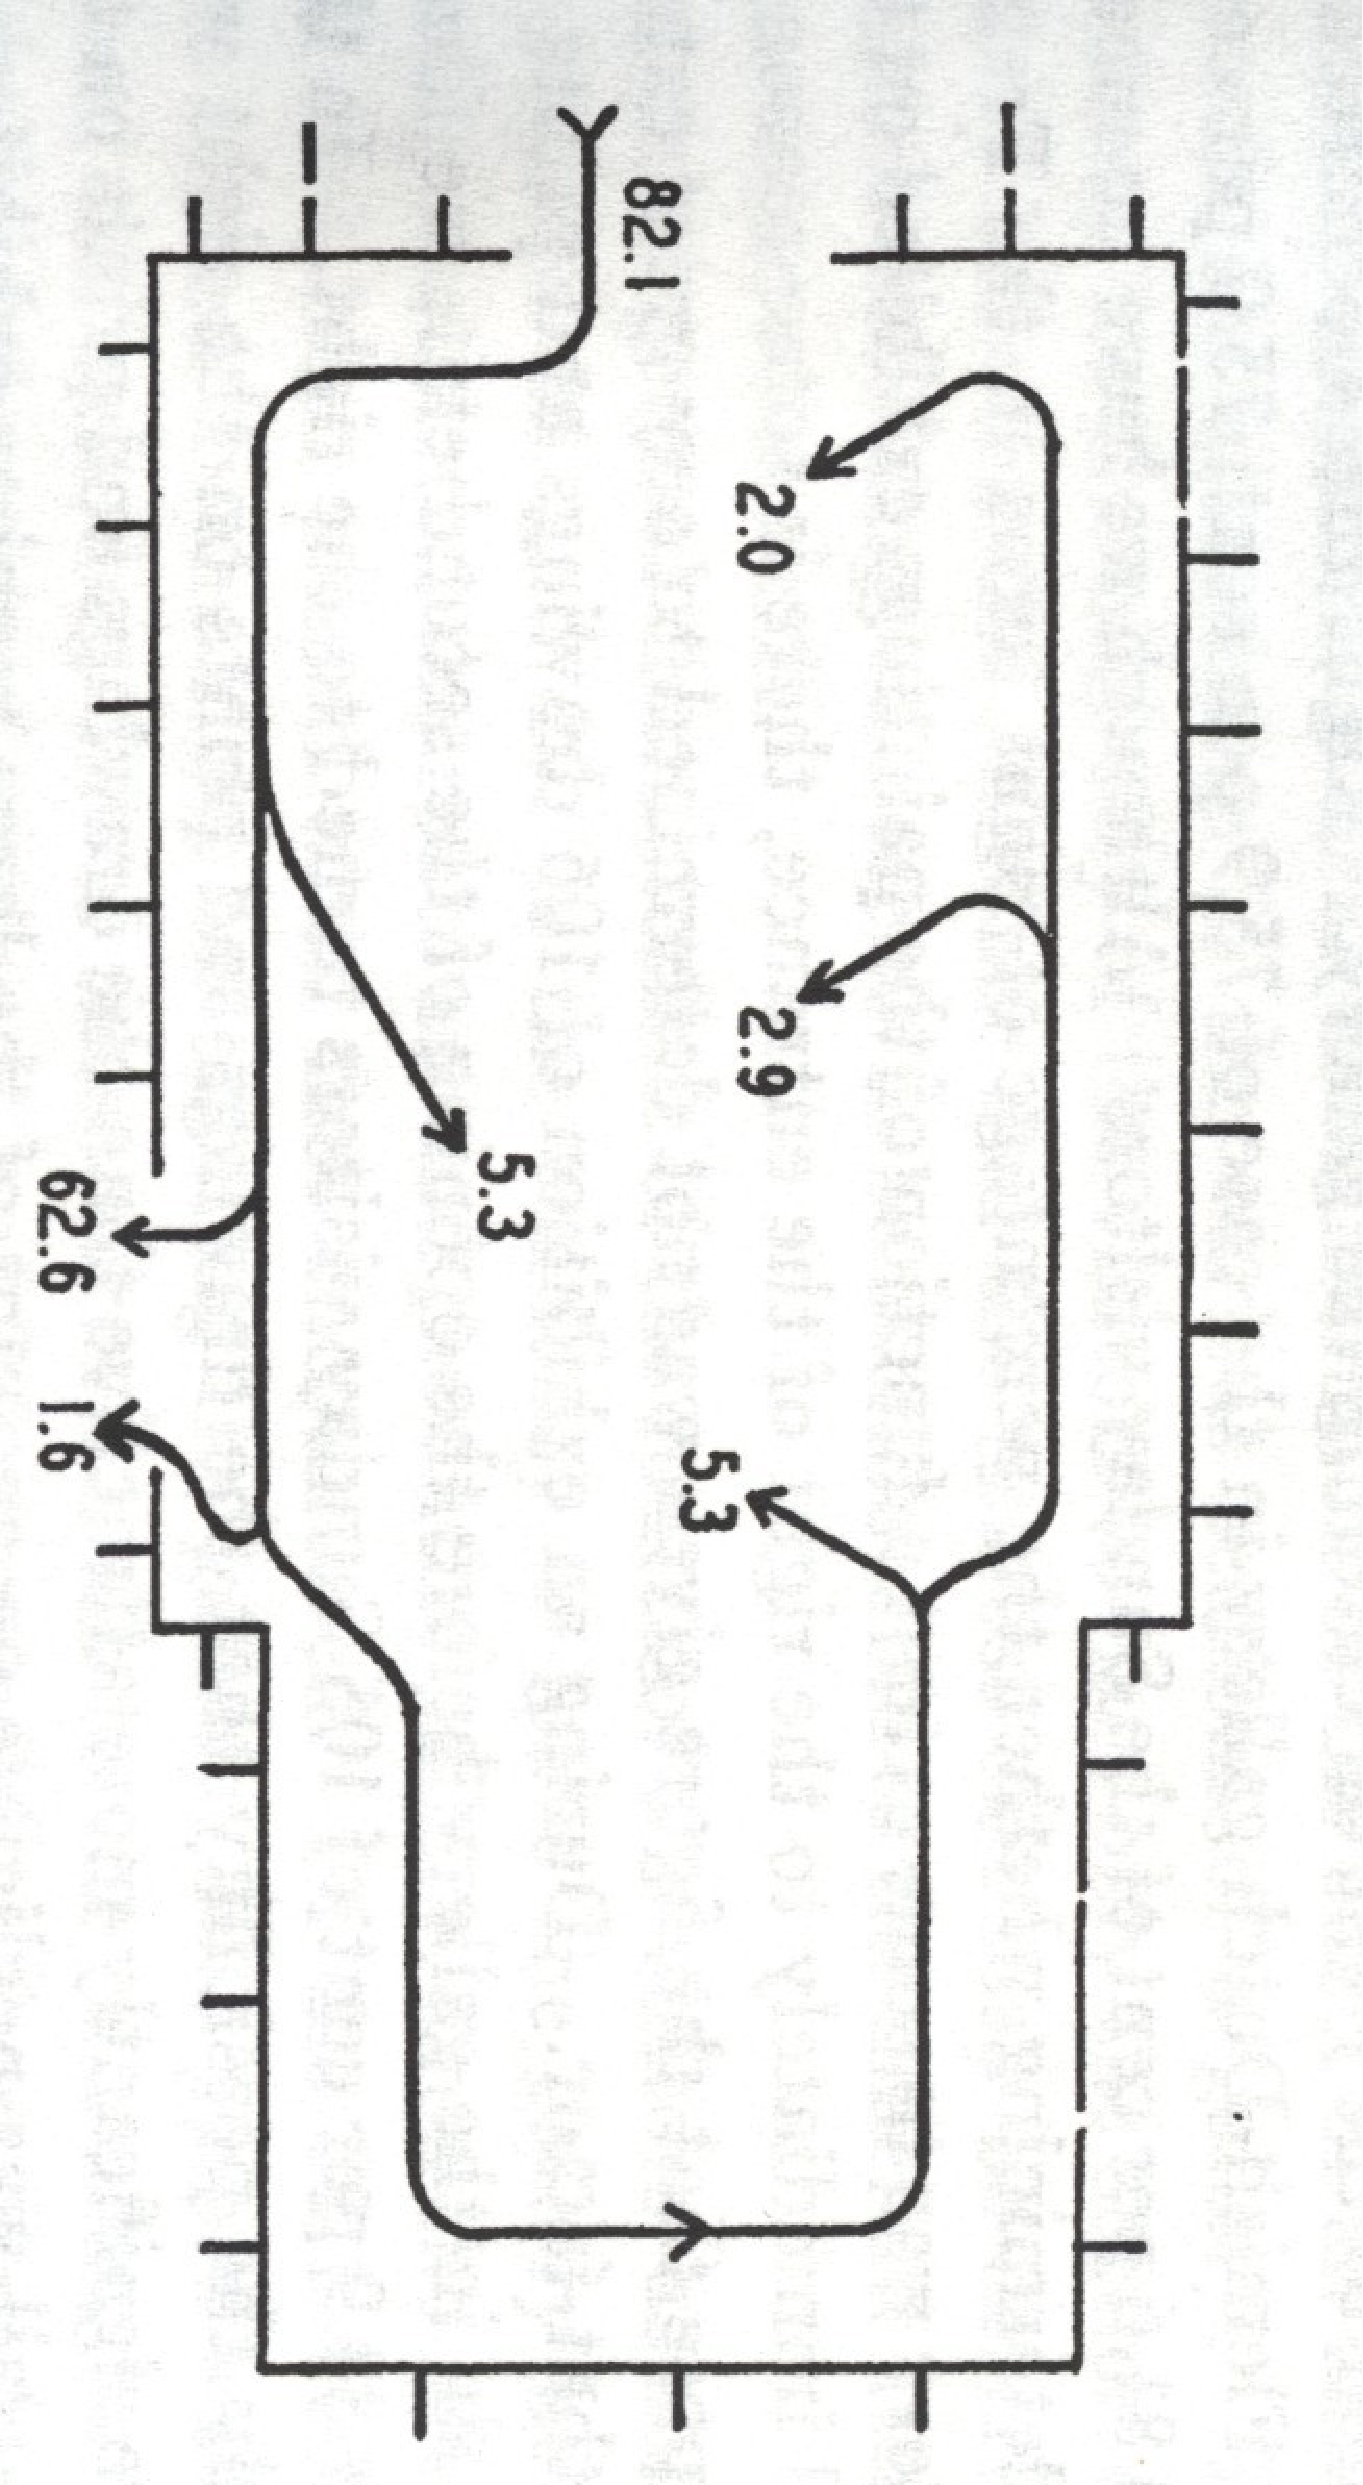
\includegraphics[width=35mm, angle=90]{melton-circulation}}
 \hspace{10 mm}
 \subfloat[frequency of visits]{\label{fig:door-opposite}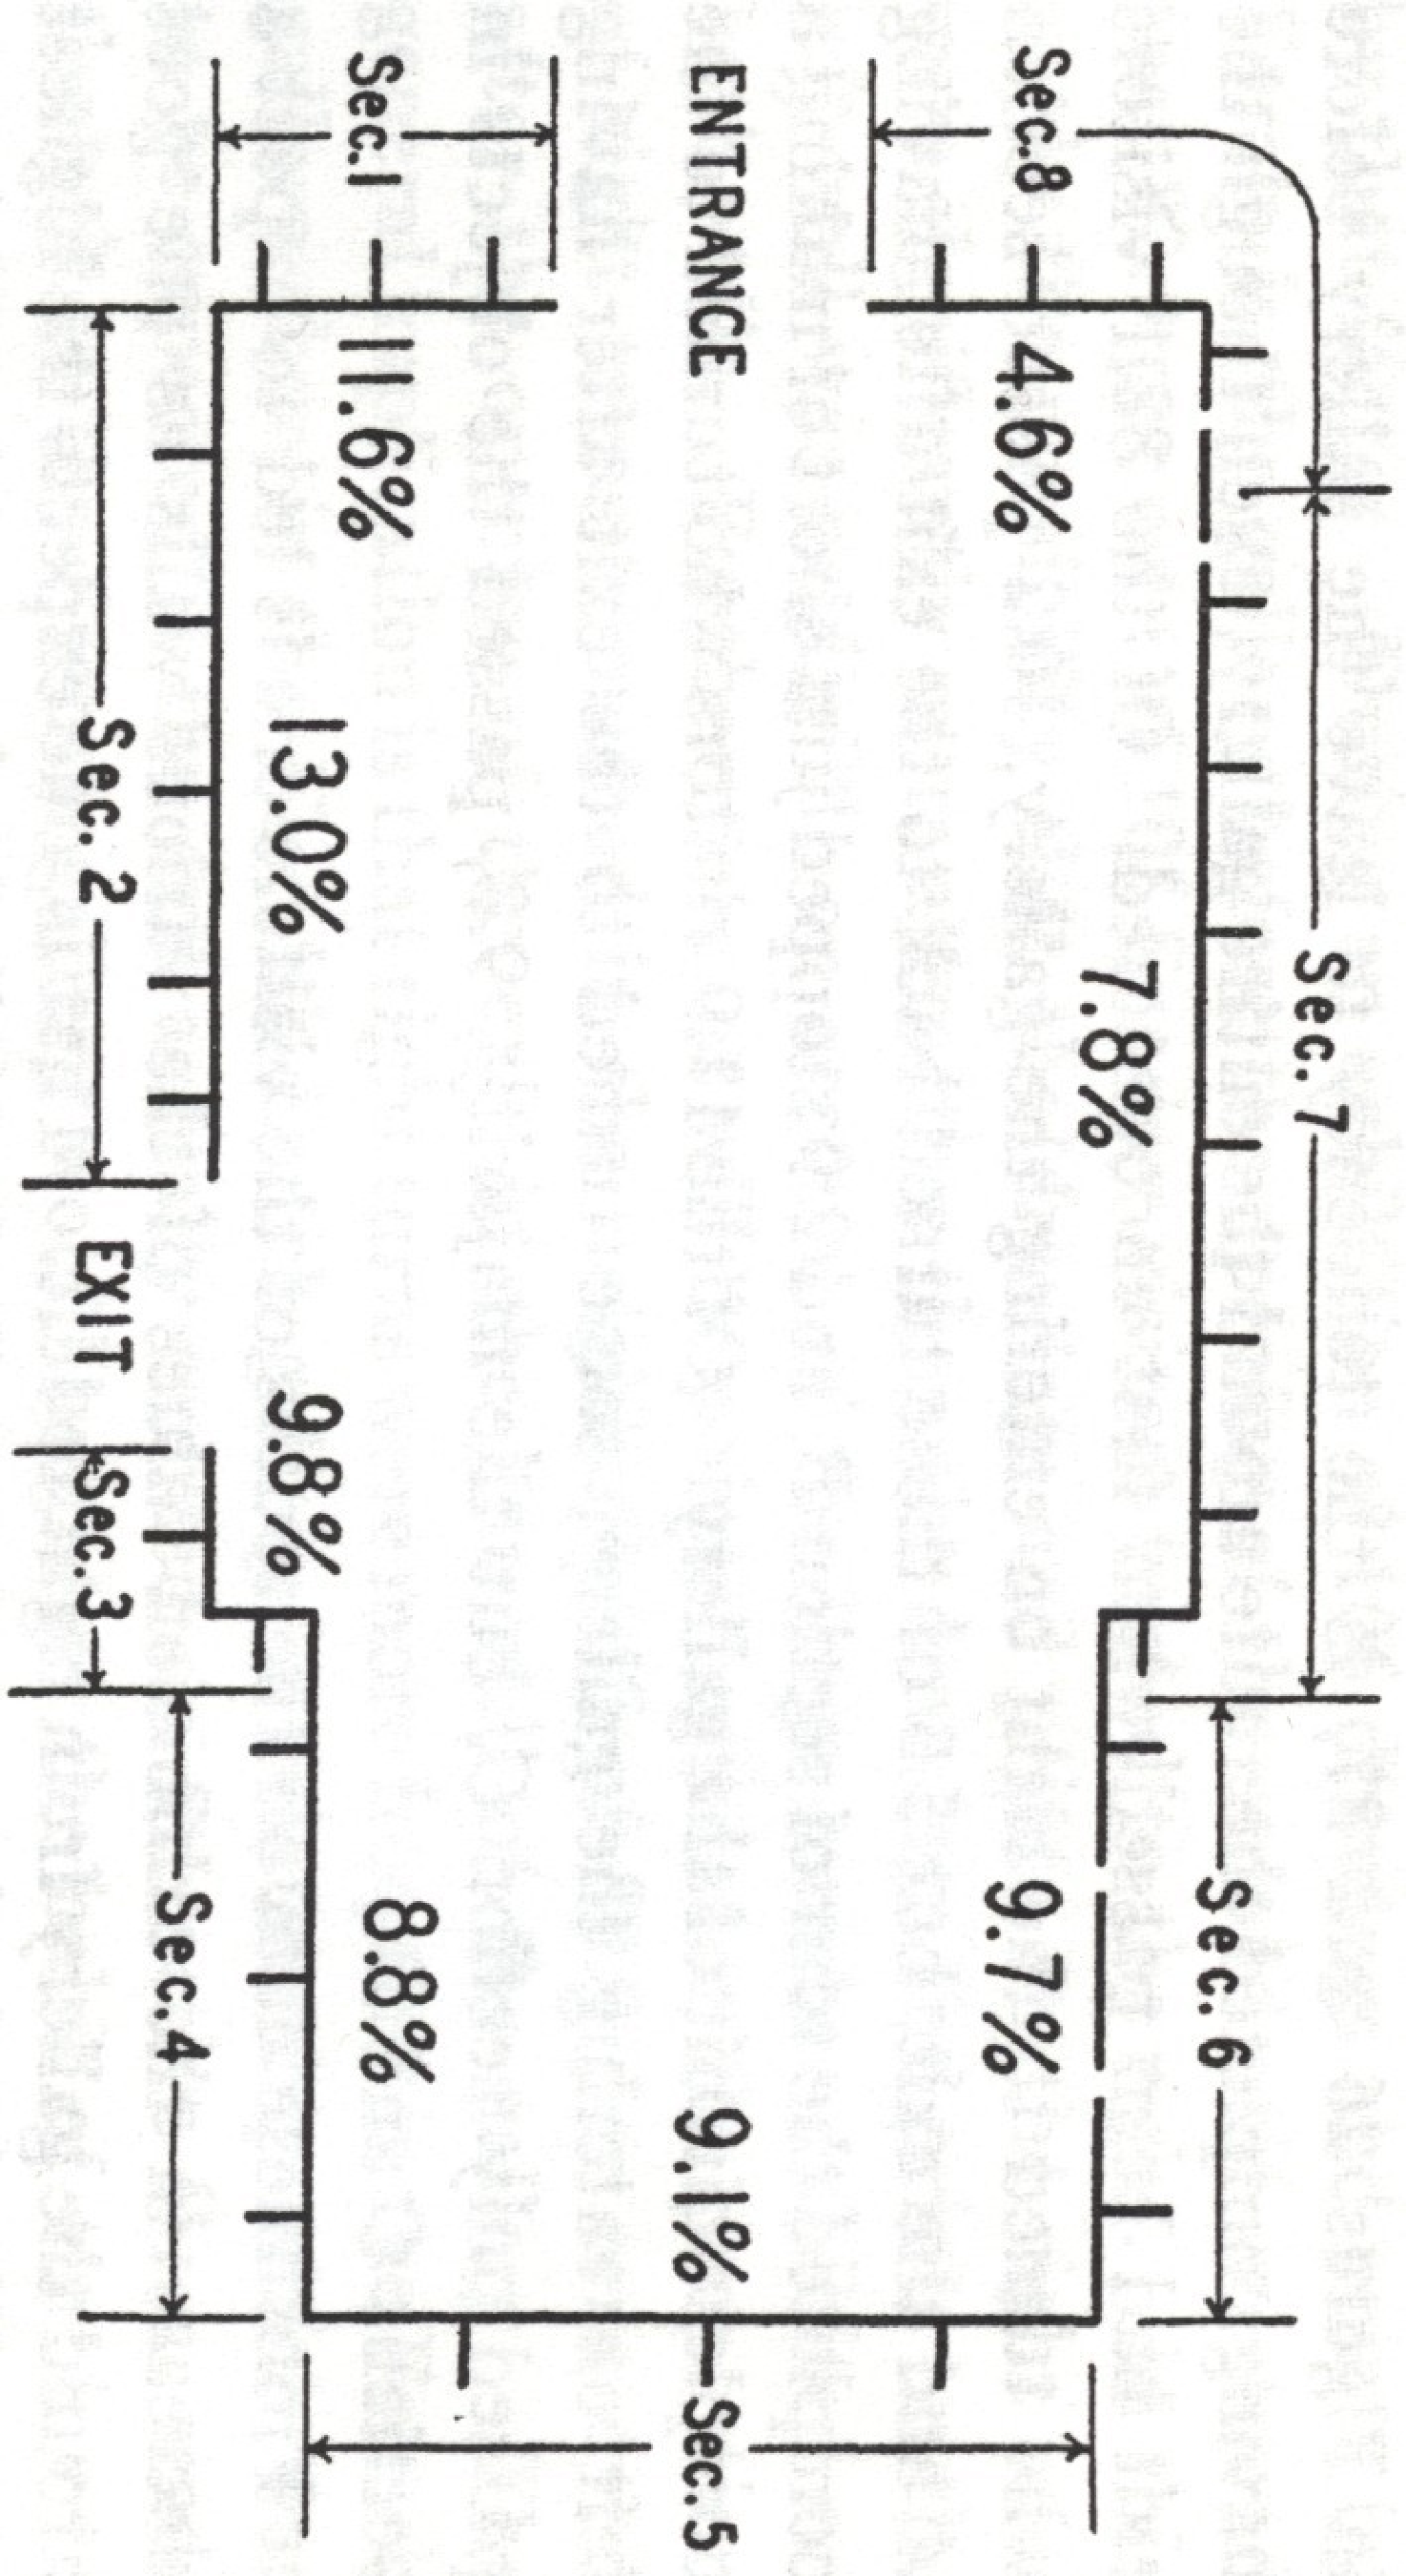
\includegraphics[width=35mm, angle=90]{melton-frequency}}
 \label{melton}
 \caption{Results from Melton's experiments on the effects of door positioning in an Art Museum}
\label{Melton-studies}
\end{figure}

The crux of Melton's experiments suggested that visitors exit through the first door they encounter, which he referred to as the exit gradient. Figure \ref{Melton-studies} shows the results of an extensive study of visitors circulation patterns and stopping frequencies in an art museum. The studies reported that almost 80 percent of visitors exited through the first exit they encountered before viewing the entire exhibition. Additionally, the studied showed that the most frequently visited objects where those located along the shortest path from the entrance to the exit. 

The results of Melton's studies inform architects of spatial characteristics that influence movement patterns in exhibitions. Specifically, doorways that are positioned on the same side of the room cause visitors to pay attention to fewer exhibits than doorways that are positioned on opposing sides of the room.

\begin{description}
\item[Requirement 1:] Exhibition doorways should be positioned on opposing sides of gallery rooms. 
\end{description}

Figure \ref{door-position} shows a possible exhibition design where the red door is positioned on the same side of the room as the entrance, while the black door is positioned on the opposing side.
\begin{figure}[H]
\centering
\subfloat[consistent design]{\label{fig:door-opposite}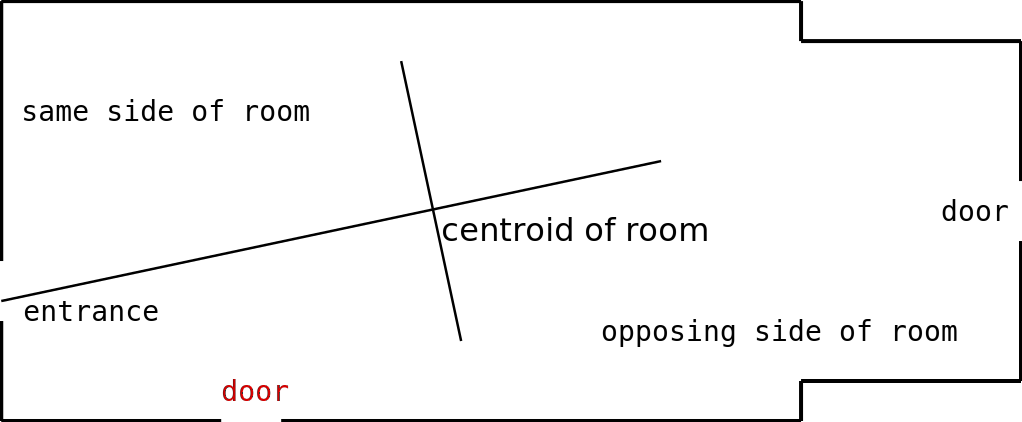
\includegraphics[width=85mm]{door-possitioning}}
\caption{Schematization of the opposing door requirement.}
\label{door-position}
\end{figure}

Bitgood suggests that visitors tend to follow along the wall that is closest to the door they entered \cite{Bitgood95}. Given that visitors also tend to exit through the first doorway they encounter, doorways should not be positioned in a wall that is adjacent to another doorway.  
 
\begin{description}
\item[Requirement 2:] Exhibition doorways should not be positioned on a wall that is adjacent to another doorway.
\end{description}


\subsubsection{Spatial arrangement of display cases}
The spatial arrangement of display cases in galleries has been shown to influence visitors' movement patterns. \cite{Bitgood92} showed that display case arrangements that form a perimeter or a peninsula generate the most amount of attention, while display case arrangements that form an island in the middle of the room received the lowest amount of attention.

   \begin{figure}[H]
 \centering
 \subfloat[island]{\label{fig:door-opposite}
\includegraphics[width=35mm]{island}}
 \hspace{10 mm}
 \subfloat[perimeter]{\label{fig:door-opposite}
\includegraphics[width=35mm]{perimeter}}
  \hspace{10 mm}
 \subfloat[peninsula]{\label{fig:door-opposite}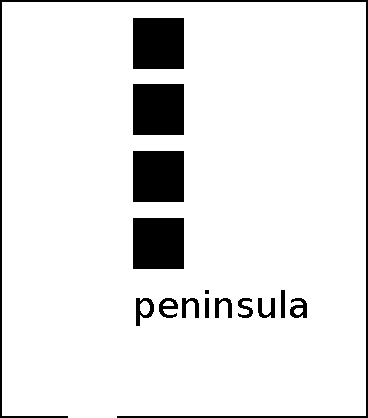
\includegraphics[width=35mm]{peninsula}}
 \caption{Display case arrangements}
\label{display-arrangement}
\end{figure}
 
\begin{description}
\item[Requirement 3:] Display case arrangements should not form an island near the center of the room.
\end{description} 

Circulation patterns can be disrupted when a peninsula arrangement cuts horizontally across the view of a visitor as they are entering the room. This type of display pattern will cut off part of the room from the visitor and will make it less likely to be visited.

\begin{description}
\item[Requirement 4:] Display cases arrangements that form a peninsula should not cut horizontally across the view of a visitor located at an entrance.
\end{description} 

\begin{figure}[H]
\centering
\subfloat[consistent design]{\label{fig:door-opposite}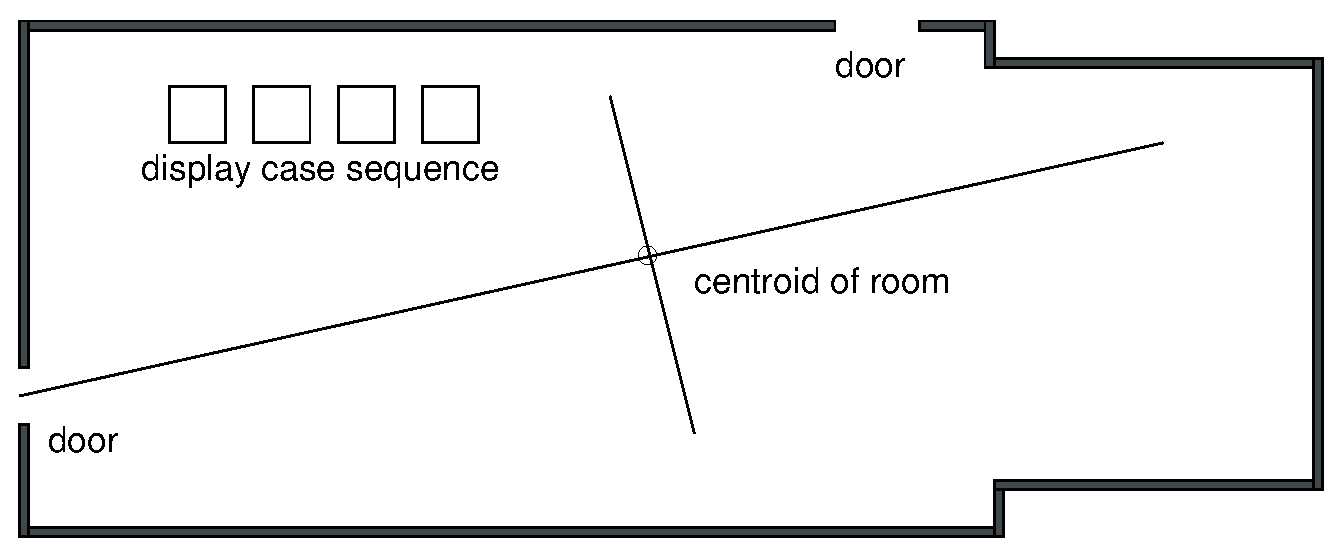
\includegraphics[width=65mm]{display-not-cut}}
\hspace{10 mm}
\subfloat[inconsistent design]{\label{fig:door-opposite}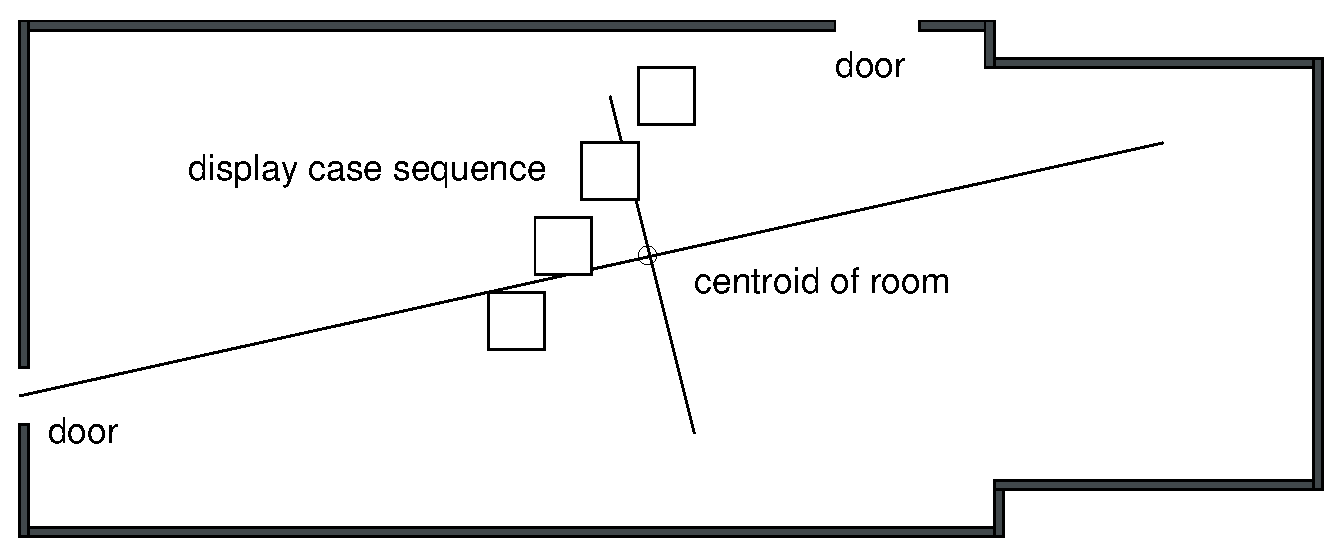
\includegraphics[width=65mm]{door-cut-room}}
\end{figure}


\subsubsection{Congestion}
Congestion in museums can be caused by interference of displayed objects and their viewing spaces with movement pathways of visitors. In order to reduce congestion in museums, designers should be aware of the placement of display cases, statues, furniture (seating benches), and information kiosks within the gallery. The following are requirements that should be followed to reduce congestion in museums:

\begin{description}
\item[Requirement 5:] The viewing area of display cases, functional space of doors, function space of seating areas, and operation space of information kiosks should not interfere with each other.
\end{description}

\subsubsection{Positioning of benches, statues, and information kiosks}
The positioning and orientation of benches and statues can increase the amount of attention an exhibition receives and change circulation patterns within a gallery \cite{Stavroulaki} \cite{Museum}. Studies have shown that seating directly facing an object will increase the attention the object receives, even if no one uses the seating. 

\begin{description}
\item[Requirement 6:] Seating should directly face a gallery wall or display case.
\end{description}

The orientation of a statue to doorways can increase the attention the statue receives as well as the object close to it. Statues that face away from doorways encourage visitors to move around the statues in order to get a better view.  
\begin{description}
\item[Requirement 7:] Statues should face away from doorways.
\end{description}

\subsubsection{Visitor Orientation in the lobby}
The lobby is the first place visitors encounter when they enter a museum. The design of the lobby is important because it not only provides a first glimpse of the museum's exhibits but it is the place where the museum provides services to its visitors, including: a ticketing desk, bathrooms, an information desk, and entrances to exhibitions \cite{Bitgood02}. The aim of the requirements for the lobby focus on making it easy for visitors to locate services and orient themselves to the new environment. 

Upon entering the lobby most visitors need to find the ticket area and/or an information desk. It is important, therefore, that the ticketing area and information desk are visible from the entrance. If there is more then one entrance, then it is important that the ticket area and information desk are visible from all entrances. 

\begin{description}
\item[Requirement 8:] The ticketing and information desks should be visible from the main entrance(s).
\end{description}

Additionally, studies have shown that people first look to their right hand side when entering a building. By placing the ticket and information desks on the right hand side of the lobby, visitors are more likely to notice them immediately when they enter the lobby. 

\begin{description}
\item[Requirement 9:] The ticketing area should be on the right side of the lobby from the main entrance(s).
\end{description}

The ticketing area should be close to visitors when they enter because it is likely one of the first places they will need to visit.
\begin{description}
\item[Requirement 10:] The ticketing are should be on the same side of the lobby as the entrance(s).
\end{description}

Bathrooms are an important services for museum visitors. Surprisingly, the place of the bathroom can have an impact on how long visitors stay in the museum. Studies \cite{tbd} have found that bathrooms that are located on the same side of the lobby as the entrance / exit encourage visitors to leave earlier compared to museums with bathrooms on the opposing side of the lobby from the entrance / exit. 

\begin{description}
\item[Requirement 11:] The bathroom should be on the opposing side of the lobby from the entrance / exit.
\end{description}

The doors should be private to maintain as much privacy in the bathrooms as possible.

\begin{description}
\item[Requirement 12:] Bathroom doors should be private.  
\end{description}

The main exhibition entrance should be clearly visible from several parts of the lobby to make it easy for visitors to find where they need to go. 
\begin{description}
\item[Requirement 13:] Exhibit entrance should be visible from the ticketing area and central lobby location
\end{description}


\subsection{Exploration}
The way visitors explore an exhibition is influenced by the spatial characteristics of the layout, as well as the characteristics of each gallery room. Layouts that are sequential, i.e. one way in / one way out, promote a controlled and orderly flow of movement. Museums of history and science are well served by this type of design because they have a narrative to tell that is chronological. On the other hand, layouts that present the visitor with path choices, i.e. multiple doorways, promote free-flowing exploration. In this type of layout it is important that visitors are aware of the path choices that are available. This means that doorways are visible between each other throughout the layout. This concept of visibility between a network of points is referred to as continuity and is an important characteristic of layouts that present visitors with multiple path choices.  

\begin{description}
\item[Requirement 14:] The layout of the museum should maintain continuity between doorways within each exhibition and gallery room.
\end{description}

Within a Gallery, rooms that are open promote more free-flowing exploration than rooms that are narrow. Narrow rooms inhibit exploration because of space limitations and confinement. Rooms that are open provide more space for visitors to explore the room in a free-flowing manner.
\begin{description}
\item[Requirement 15:] Gallery rooms should be open, rather than narrow, in order to promote free-flowing exploration.
\end{description}


\subsection{Accessibility and Security}
Museums should be accessible and easy to navigate. TBD - I have some ideas here but nothing concrete. Maybe you have some ideas that you can share with me. 
\begin{description}
\item[Requirement 16:] Museums should be accessible.
\end{description}
Museums should be secure.
\begin{description}
\item[Requirement 17:] The functional space of every gallery doorway should overlap with the range space of at least one security camera.
\end{description}


\section{Representation and Reasoning for Museums of Art in DSpace} 


\subsection{Representation}

\subsubsection{Spatial Interpretation of a Design Requirement}

\subsubsection{Using the Building Blocks from DSpace}

\subsection{Case Study Tests}

\subsubsection{ArchiCAD / IFC}

\subsubsection{Detecting Inconsistent and Consistent Designs}

\chapter{Evaluation}


\chapter{Future Work / Conclusion}



% ------------- End main chapters ----------------------

\clearpage
\bibliographystyle{abbrv}
\bibliography{museum}
%\bibliography{architecture}
\bibliography{qsr}
%\bibliography{clp}
%\bibliography{relatedworks}

%\addcontentsline{toc}{chapter}{Bibliography}

\end{document}